\documentclass{report}


% Language + Document formatting
\usepackage[dutch]{babel}
\usepackage[a4paper,top=2cm,bottom=2cm,left=2cm,right=3cm,marginparwidth=1.75cm]{geometry}
\usepackage[indent=10pt]{parskip}

% Titles customization
\usepackage{titlesec}
\newcommand{\hsp}{\hspace{20pt}}
\titleformat{\chapter}[hang]{\Huge\bfseries}{\thechapter\hsp}{0pt}{\Huge\bfseries}


% Afbeeldingen
\usepackage{graphicx}
\graphicspath{ {./images/} }


\title{OnlyPaws}
\author{Mathijs Verbeure}

\begin{document}
\maketitle

\tableofcontents

\chapter{Inleiding}
De eerste vraag wanneer een project zo absurd als ``een dating platform voor katten'' gepresenteerd wordt is: \verb|Waarom?| Een concreet antwoord hierop\dots heb ik niet.
Toen het project voorgelegen werdt nam ik de beslissing om geen standard onderwerp te nemen. Wat brutaal gezegd: niks saai.
Zo behoud ik mijn motivatie en valt de kraan niet zo snel dicht.
Een ander punt waar ik rekening mee nam was dat dit project, indien mooi afgerond, leuk op een CV / Portfolio kan komen. 
Kotlin is een snel evoluerende taal die veel gebruikt wordt binnen de Google-omgeving, en zeker toegepast kan worden binnen de context van een bedrijf.
Een topic kiezen die interessant is en waarover veel te bespreken valt is dus erg belangrijk; veel valt er niet te vertellen over een \verb|To-Do| app, maar een online dating app voor poezen? Dat lokt wel aandacht!

Dit waren dus de officiële redenen voor dit project, maar er blijven er nog twee over die het meeste invloed gehad hebben op mijn beslissing. 
\begin{enumerate}
    \item Ik heb poezen graag; het zijn grappige beesten.
    \item Het is een grappig concept.
\end{enumerate}


\textit{OnlyPaws} is gebaseerd op \textit{Tinder}\texttrademark, het online dating platform. Hier kunnen gebruikers profielen bekijken van andere, naar rechts swipen indien de persoon hun interesseert en naar links indien niet.
Indien beide gebruikers naar rechts swipen --- zal ik verder ``Liken'' noemen --- dan is het een ``Match'', en kunnen ze berichten naar elkaar sturen om verder contact op te nemen.

Een vrij simpel concept dat enorm populair is geworden. Zelf had ik \textit{Tinder} nog nooit gebruikt, enkel via een vriend of het internet de groffe lijnen begrepen.
Om een app te ontwerpen hierrond moest ik uiteraard zelf eens uit proberen en notities nemen over de UI/UX.\@ De `testprocedure' was inzichtsvol en bracht verschillende ideeën op die ik zou proberen te integreren in mijn versie.
Sommige details in de UX vielen erg hard op, zoals bij voorbeeld hoe vaak er een voorstel komt om een subscriptie te nemen die je voordelen geeft. Eens je maandelijks betaal kan je berichten sturen zonder match --- via wat ze ``First Impressions'' noemen --- bekijken wie jouw profiel geliked heeft en meer.
Al zou het hilarisch zijn om tijdens de demonstratie niks te kunnen tonen omdat er betaald moet worden, dit zal ik voor overduidelijke redenen niet doen. 

De economische strategieën van techgiants zijn niet te bespreken in dit verslag. Dit is een project in academische context, geld-gerichte implementaties zijn dus niet gepast.
Verder nog, zelf vind ik dat bedrijven veel te gericht zijn op winst, niet op de producten die gemaakt worden; \textit{Tinder} valt amper te gebruiken door alle reclame die ingebouwd is. Dit weiger ik op eender welke wijze te implementeren.

Deze negatieve kanten van het oorspronkelijk product zijn dus niet te vinden in dit project --- en meer zelfs! Deze verschillen bespreek ik wel eens ze aan bod komen.


\chapter{Verloop}

Bij het openen van de app gaat Google's \textit{Credential Manager} open. Deze onthoudt welke gegevens al gebruikt zijn om in te loggen of te registreren.
Dankzij deze moet je je paswoord ook niet onthouden; het wordt allemaal veilig bewaard door Google.
De pop-up laat je selecteren welk account je wilt gebruiken als, stel maar, je meerdere katten hebt. Indien er geen credentials te vinden zijn wordt je automatisch naar de Register pagina verstuurd.
Verder kan je ook het Credentials menu sluiten om een gebruiker aan te maken.

Het proces om een gebruiker aan te maken neemt twee stappen, gesplitst over twee opeenvolgende paginas; eerst de belangrijke gegevens voor login, dan de informatie die andere gebruikers zullen zien.
Je vult een email in, gevolgd door een paswoord. Je mag door naar de volgende stap eens deze checks goedgekeurd zijn: het emailadress mag nog niet in de database bestaan en het paswoord moet meer dan 6 karakters lang zijn.
In een perfecte wereld zou een bevestigingsmail verstuurd worden, maar dat valt buiten de scope van dit project.

In de tweede pagina moet je een naam, beschrijving en afbeelding invullen, die andere gebruikers te zien krijgen. Er zijn geen beperkingen op deze, alleen ze mogen niet leeg zijn.
Hier komt de scope van dit project weer in spelen: ik maak gebruik van Firebase RealTime database om alle gegevens en authenticatie op te slaan. Hier kunnen geen afbeeldingen opgeslaan worden, alleen text/JSON.
Daarom zijn er op de RegisterDetails pagina twee knoppen; één om een afbeelding lokaal te openenen en één waarbij je de link naar een random foto online krijgt. 
Beide zijn volledig functioneel, maar de lokale afbeelding gaat door niemand buiten de huidige telefoon bekeken kunnen worden, dus raad ik niet aan.

Proficiat! U bent nu de trotse eigenaar van een OnlyPaws account en wordt doorgestuurd naar de Home pagina.
Hier worden één per één andere profielen getoond. Je kan ofwel Liken ofwel Disliken, door rechts of links te klikken op de pagina. 
Centraal staat de foto van de kat met de naam en beschrijving bovenaan.
Elke profiel die geliked wordt komt in de Favorites pagina te staan. Hier kan je alle profielen van Liked naar Dislike sturen en omgekeerd, plus de foto's bekijken door op de thumbnail te klikken.
Bij het verwissellen van een profiel komt een pop-up tevoor om na te vragen of de gebruiker dit zeker wilt doen. Indien ja, wordt de operatie uitgevoerd. Indien nee sluit de pop-up en verandert er niks.

Ten laatste is er een Account pagina, waar de gebruikersgegevens aangepast kunnen worden. Een lokale foto opslaan kan nog niet, dus de profiel foto aanpassen is nog niet mogelijk, maar naam en beschrijving wel.
Voer de nieuwe text in, duuw op het knopje en de gegevens worden opgeslaan.
In de boven-rechtse hoek is een Log-Out knop te vinden waarmee je, uiteraard, kunt uitloggen van het account en terug naar de Login gaan.


\chapter{Documentatie}
\section{MVVM}
MVVM is een structuur waarbij er zo veel mogelijk abstractie is tussen data en display. Doorheen het process is de structuur meerdere keren vanaf nul weer begonnen,
vaak omdat ik een nieuwe manier van werken gevonden had en die voorkeur gaf over de oude methode.
Een van de belangrijkste concepten is het \textit{Separation of Concerns} principe. Dit legt voor dat elk object, elke classe, elke pagina, elk data model geen kennis mag hebben van waar het gebruikt wordt, of in welke toepassing het beland.
Eender welk bestand zou theoretisch geplakt kunnen worden in eender welke omgeving en werken. Een pagina zou geen fout moeten geven als een viewmodel verwisselt wordt.
De structuur die ik aangenomen heb voor dit project draait om een paar begrippen die bij elke toepassing opnieuw gemaakt worden,
en op een robuste manier code veiligheid behalen.


\subsection{ViewModel}
Viewmodels zijn de classes waarin data wordt bijgehouden. Ze doen het rekenwerk, halen data op en sturen de nodige informatie door naar de gebruikersinterface.
Intern bestaan er meerdere variabelen die doorheen de levenstijd van het viewmodel geldig blijven, samen met de nodige functies om alles operationeel te krijgen.
Verder is er maar één publieke property --- de ScreenState --- en één publieke methode --- de OnAction methode. Meer hierover in het Action subsectie.

Het basis ViewModel classe heeft twee eigenschappen die nodig zijn voor hun verwachtte werking.
De eerste hiervan is dat ze niet composable zijn; hierdoor moet er geen \textit{remember} toegevoegd worden zodat ze heen de lifecycle van de applicatie blijven.
Dit werkt samen met de tweede eigenschap: ze volgen het singleton patroon. Dit garandeert dat elke nieuwe aanroeping van een VM identiek hetzelfde object zal geven.
Aan de hand van deze twee eigenschappen kunnen VMs doorheen de levenscyclus van de applicatie geldig blijven.




\subsection{Screen}
Screens vormen de omgeving waarmee de gebruiker kan interageren. Dit zijn de ``views'' van in het MVC patroon.
Het toont de gegevens op één manier ongeacht welke gegevens dit precies zijn. 
Al wat de Screen weet is dat er een dataset gegeven wordt in een zeker formaat en dat er een zeker stuk code uitgevoerd moet worden bij het klikken op de knop.
Nogmaals, dit is een manier om de taken binnen de applicatie te splitsen. Wat het klikken op een knop doet maakt de Screen volledig niets uit. Of dit een externe library ophaalt, data schrijft naar een bestand of een Toast aanmaakt is irrelevant.
Alles wat een component hoort te weten is dat er een functie bestaat bij het klikken van elke knop.

Aan de hand van de huidige state parameter wordt de correcte display vooruit gebracht.
Elke screen heeft één publieke constructor en verschillende privé constructoren die voor de verschillende scenario's dienen.
Zo zijn er standard een ``Success(value)'', ``Failure(error)'' en ``Loading'', drie vaak voorkomende scenarios.

\begin{center}
    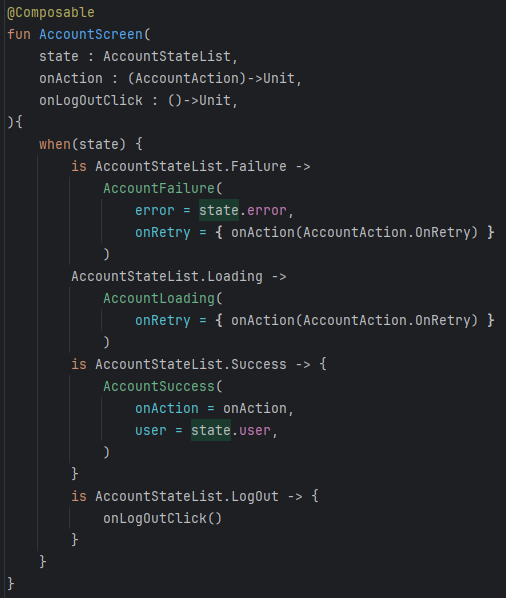
\includegraphics{Screen_state}
\end{center}

\subsection{State}
State object zijn bundles waarmee alle nodige informatie voor de screens wordt gegeven.
Er wordt gebruik gemaakt van Kotlin's sterke enum types om verschillende mogelijkheden efficiënt te behandelen. Elke entry is een data class/object heeft andere parameters.
Zo weet de Screen dat een Failure entry een foutmeldingsstring bevat, terwijl een Success entry bvb. een CatProfile heeft.
De publieke constructor van de screens krijgen een state als parameter vanuit het viewmodel en lossen intern elke entry op met een aparte composable functie.

Stel er wordt externe data opgehaald door het viewmodel, en er loopt iets mis. Het viewmodel kan een Failure state inzetten met een foutmelding.
Dit belandt bij de Screen en deze kan verder met de correcte privé constructor.


\begin{center}
    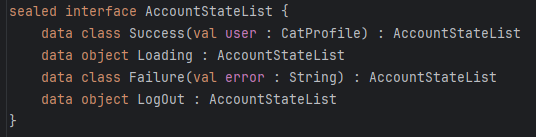
\includegraphics{VM_State}
\end{center}



\subsection{Action}

Het Action object, waarmee de Screen acties kan laten uitvoeren in het viewmodel.




\section{Database}

\section{Navigatie}

\end{document}